\documentclass[14pt, a4paper]{extreport}

% Constant
\newcommand{\CourseTitle}{Програмування комп'ютерних та віртуальних мереж}
\newcommand{\Variant}{5}
\newcommand{\StudentGroup}{ІМ-51мн}
\newcommand{\CourseNumber}{1}
\newcommand{\StudentName}{Ковальов Олександр}
\newcommand{\Teacher}{доцент, Долголенко Олександр Миколайович}
\newcommand{\Year}{2025}
% Variable
\newcommand{\LabNumber}{3}
\newcommand{\Topic}{Створення лінійної SDN мережі на базі OpenFlow}
\newcommand{\SubmissionDate}{16.10.2025}

\usepackage{caption}
\usepackage{enumitem}
\usepackage{fancyhdr}
\usepackage{float}
\usepackage{fontspec}
\usepackage{geometry}
\usepackage{graphicx}
\usepackage{hyperref}
\usepackage{hyphenat}
\usepackage{indentfirst}
\usepackage{listings}
\usepackage{polyglossia}
\usepackage{setspace}
\usepackage{unicode-math}
\usepackage{xcolor}



\defaultfontfeatures{Ligatures=TeX}
\graphicspath{{./images/}}
\fancyhf{}
\hypersetup{unicode=true, colorlinks=true, linkcolor=black, urlcolor=black}
\pagestyle{fancy}
\setlength{\headheight}{18pt}
\setmainfont{Times New Roman}
\setmathfont{Latin Modern Math}
\setmonofont[Scale=0.8]{DejaVu Sans Mono}
\setotherlanguage{english}
\setsansfont{Arial}
\onehalfspacing

\renewcommand\headrulewidth{0pt}
\cfoot{\thepage}

\geometry{
	a4paper,
	left=25mm,
	right=10mm,
	top=15mm,
	bottom=15mm,
}

\definecolor{codegreen}{rgb}{0,0.6,0}
\definecolor{codegray}{rgb}{0.5,0.5,0.5}
\definecolor{codepurple}{rgb}{0.58,0,0.82}
\definecolor{backcolour}{rgb}{ 0.976, 0.976, 0.976 }

\lstdefinestyle{mystyle}{
	backgroundcolor=\color{backcolour},   
	commentstyle=\color{codegreen},
	keywordstyle=\color{magenta},
	numberstyle=\tiny\color{codegray},
	stringstyle=\color{codepurple},
	basicstyle=\ttfamily\footnotesize,
	breakatwhitespace=false,         
	breaklines=true,                 
	captionpos=b,                    
	keepspaces=true,                 
	numbers=left,                    
	numbersep=5pt,                  
	showspaces=false,                
	showstringspaces=false,
	showtabs=false,                  
	tabsize=2
}

\lstset{style=mystyle}

\setlist[enumerate]{
	itemsep=0.0\baselineskip,
	left=1.25cm,
	rightmargin=10mm,
	labelsep=0.5cm,
	listparindent=1.25cm,
	parsep=0pt
}


\begin{document}
	\tolerance=350 % Or just increase the number
	\emergencystretch=3em
	
	\begin{titlepage}
		\begin{center}
			{Національний технічний університет України\\
				«Київський політехнічний інститут імені Ігоря Сікорського» \\[1.0em] }
			{Факультет інформатики та обчислювальної техніки\\}
			{Кафедра обчислювальної техніки \\[5.0em]}
			
			{\textbf{ЗВІТ}\\[1em]}
			{\textbf{з лабораторної роботи №\LabNumber} \\}
			{\textbf{з дисципліни "\CourseTitle"} \\[2.0em]}
			
			{\textbf{Тема: \Topic} \\[2.0em]}
			
			{\textbf{Варіант №\Variant} \\[5.0em]}
			
			\begin{flushright}
				Виконав: \\
				Студент \CourseNumber{} курсу, групи \StudentGroup \\
				\StudentName \\[2.0em]
			\end{flushright}
			
			\begin{flushright}
				Перевірив: \\
				\Teacher \\[2.0em]
			\end{flushright}
			
			\begin{flushright}
				Дата здачі: \SubmissionDate \\[5.0em]
			\end{flushright}
		
			\vfill
			КИЇВ -- \Year
		\end{center}
	\end{titlepage}
	
	\setlength{\parindent}{1.25cm}
	
	\textbf{Мета роботи.} Налаштувати та дослідити лінійну топологію SDN мережі з кількох комутаторів і хостів, перевірити її працездатність та проаналізувати обмін OpenFlow-повідомленнями за допомогою Wireshark dissector.
	
	\textbf{Завдання:}
	Створити лінійну топологію SDN мережі, що складається з \texttt{i + 2} (де \texttt{і} - номер в списку групи) поєднаних між собою OpenFlow комутаторів, до кожного з котрих підключено по одному хосту та продемонструвати її працездатність з використанням OpenFlow Wireshark dissector.
	
	\begin{center}
		\textbf{Хід роботи.}
	\end{center}
	
	Для початку, встановимо (перевіримо чи встановлені) додаткові пакети, які можуть знадобитися для роботи.
	
	\begin{figure}[H]
		\centering
		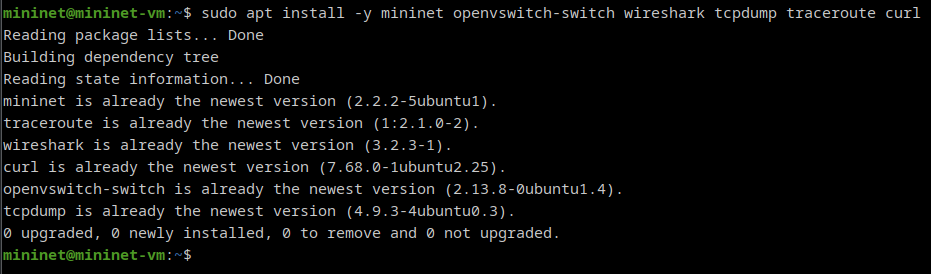
\includegraphics[height=5.2cm]{01} 
	\end{figure}
	
	За основу можна взяти скрипт з минулої лабораторної роботи. Частина з описом топології після змін виглядає так:
	
	\begin{lstlisting}[language=Python]
		def run():
			net = Mininet(controller=Controller, switch=OVSSwitch)
			c0 = net.addController('c0')
		
			variant = 5 + 2
			for i in range(variant):
				index = i + 1
				switch = net.addSwitch(f"s{index}")
				connected_host = net.addHost(f"h{index}", ip=f"10.0.0.{index}/24")
				net.addLink(switch, connected_host)
		
				if index > 1:
					previous_switch = net.getNodeByName(f"s{index-1}")
					net.addLink(previous_switch, switch)
		
			 net.start()
		\end{lstlisting}
	
	Так як варіант = 5, то потрібно створити 7 комутаторів та стільки ж хостів. Для цього використовується цикл, в якому створюються пристрої з відповідним ім'ям, а потім з'єднуються. Відповідно, була створена лінійна топологія.
	
	Далі, щоб спростити процес запуску, ще минулого разу першим рядком скрипту був встановлений "шебанг" -- вказівка, яку утиліту використовувати для інтерпретації коду:
	
	\begin{lstlisting}[language=Bash]
		#!/usr/bin/env python3\end{lstlisting}
	
	Якщо надати права на запуск за допомогою утиліти \texttt{chmod} та прапорця \texttt{-x} (executable), не треба кожного разу вказувати інтерпретатор. 
	
	\begin{figure}[H]
		\centering
		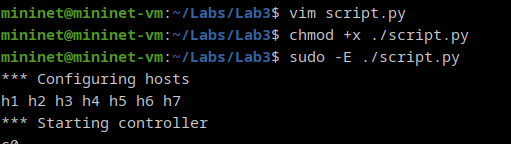
\includegraphics[height=4cm]{02} 
	\end{figure}
	
	Налаштована топологія:
	
	\begin{figure}[H]
		\centering
		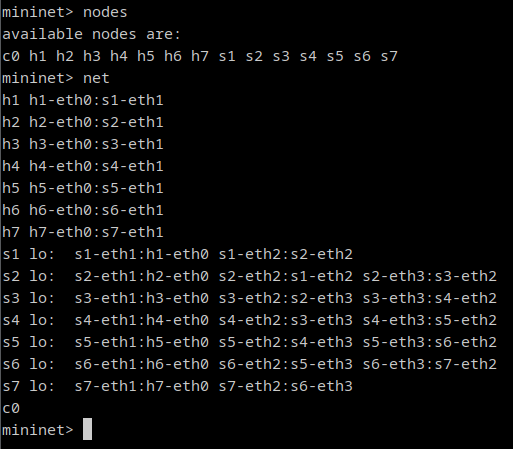
\includegraphics[height=11cm]{03} 
	\end{figure}
	
	Wireshark можна запустити командою:
	
	\begin{lstlisting}[language=Bash]
		sudo -E wireshark &\end{lstlisting}
	
	Спочатку перевіримо чи взагалі працює можливість відстежувати пакети за допомогою Wireshark. Пропінгуємо сьомий хост з першого:
	
	\begin{figure}[H]
		\centering
		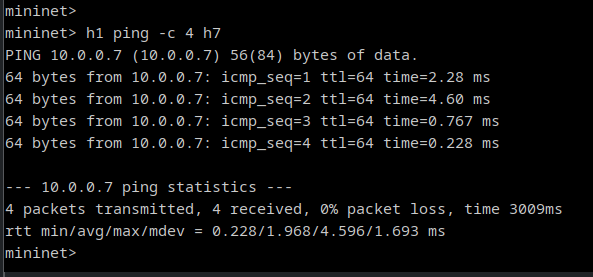
\includegraphics[height=7.5cm]{04} 
	\end{figure}
	
	Почали з'являтися пакети -- ICMP ECHO запити та відповіді. В окремих колонках можна побачити, що адреси хостів співпадають. 
	
	\begin{figure}[H]
		\centering
		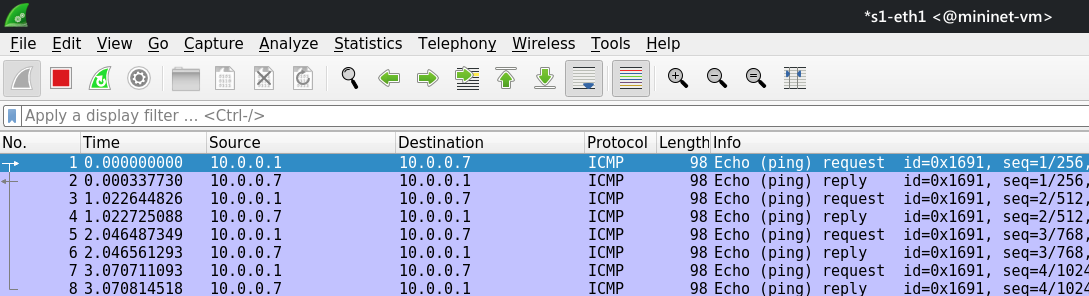
\includegraphics[height=4.5cm]{05} 
	\end{figure}
	
	Пропінгуємо знову, щоб виконати останнє завдання -- провести інспекцію пакетів, надісланих за протоколом OpenFlow. Відповідно нього, якщо на хост надходить або з нього відправляються пакети --- інформація про це надсилається за допомогою контролера.
	
	\begin{figure}[H]
		\centering
		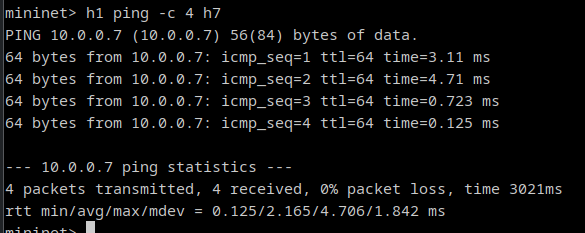
\includegraphics[height=6.5cm]{06} 
	\end{figure}
	
	Насамкінець, маємо результат -- чотири пари пакетів з типом "\texttt{OFPT\_PACKET\_IN}" та "\texttt{OFPT\_PACKET\_OUT}", які були відправлені через роботу утиліти \texttt{ping}. Також, видно джерело та призначення -- ІР-адреси хостів \texttt{h1} та \texttt{h7}.
	
	\begin{figure}[H]
		\centering
		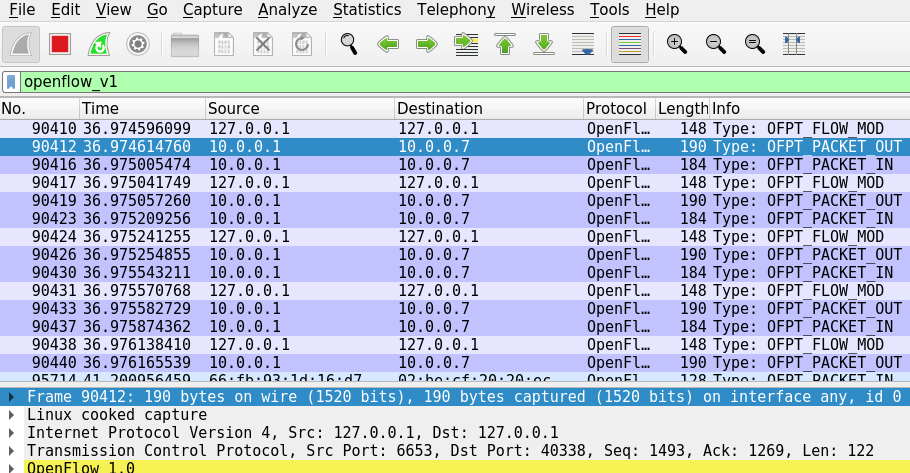
\includegraphics[height=9cm]{07} 
	\end{figure}
	
	\textbf{Висновок.}
	У ході лабораторної роботи було створено та досліджено лінійну топологію SDN-мережі, що складається із семи OpenFlow-комутаторів і семи хостів. За допомогою контролера було забезпечено зв’язок між вузлами та передано трафік між крайніми хостами. Робота мережі була перевірена за допомогою утиліти Wireshark, де вдалося проаналізувати обмін OpenFlow-повідомленнями типу "\texttt{PACKET\_IN}" та "\texttt{PACKET\_OUT}". Отримані результати підтверджують коректність налаштування SDN-топології та функціонування контролера OpenFlow.
	
	\pagebreak
	
	\begin{center}
		\textbf{Лістинг програми.}
	\end{center}
	
	\begin{lstlisting}[language=Python]
		#!/usr/bin/env python3
		from mininet.net import Mininet
		from mininet.node import Controller, OVSSwitch
		from mininet.cli import CLI
		from mininet.log import setLogLevel, info
		import os
		
		def run():
			net = Mininet(controller=Controller, switch=OVSSwitch)
			c0 = net.addController('c0')
		
			variant = 7
			for i in range(variant):
				index = i + 1
				switch = net.addSwitch(f"s{index}")
				connected_host = net.addHost(f"h{index}", ip=f"10.0.0.{index}/24")
				net.addLink(switch, connected_host)
		
				if index > 1:
					previous_switch = net.getNodeByName(f"s{index-1}")
					net.addLink(previous_switch, switch)
		
			net.start()
		
			info('*** Adding internal management port s1-mgmt with IP 10.0.0.254/24\n')
			os.system('ovs-vsctl add-port s1 s1-mgmt -- set interface s1-mgmt type=internal')
		
			os.system('ip addr add 10.0.0.254/24 dev s1-mgmt || true')
			os.system('ip link set s1-mgmt up || true')
		
			info('*** Setup complete - entering CLI\n')
			CLI(net)
			net.stop()
		
		if __name__ == "__main__":
			setLogLevel('info')
			run()
	\end{lstlisting}
		
\end{document}
